% ══════════════════════════════════════════════════════════════════════════════
% Figure captions for "Universal Spectral Matching"
% ══════════════════════════════════════════════════════════════════════════════

\begin{figure*}[!htbp]
    \centering
    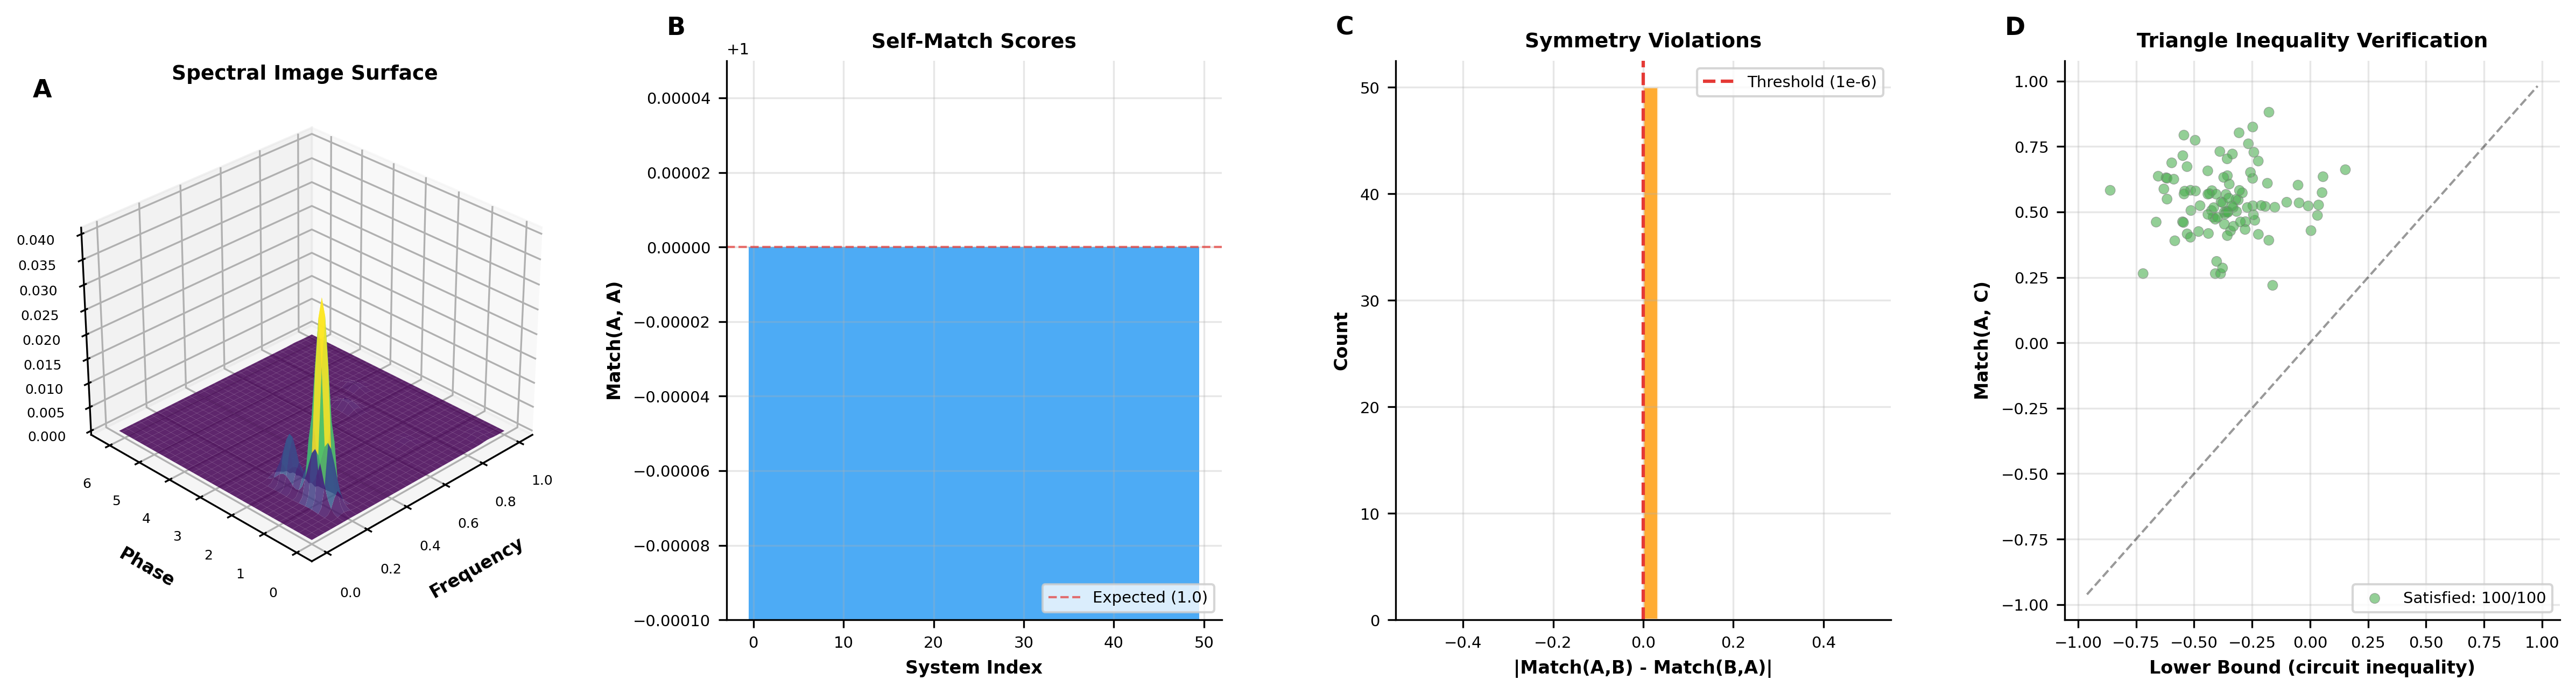
\includegraphics[width=\textwidth]{figures/panel1_spectral_image_construction.png}
    \caption{\textbf{Spectral Image Construction and Self-Consistency Validation.}
    (\textbf{A})~Three-dimensional surface plot of an example spectral image $I_X(\omega, \varphi)$ for a synthetic bounded oscillatory system with 10 frequency components. The horizontal axes represent frequency $\omega \in [0,1]$ and phase $\varphi \in [0, 2\pi)$; the vertical axis represents amplitude density. Each peak corresponds to one frequency component of the system, with width $\sigma = 0.02$ in frequency and von~Mises concentration $\kappa = 20$ in phase. The spectral image encodes the complete oscillatory fingerprint of the system as a two-dimensional intensity field---the Spectral Image Theorem (Theorem~\ref{thm:spectral_image}) guarantees this mapping is injective and metric-preserving.
    (\textbf{B})~Self-match scores $\mathrm{Match}(A, A)$ for all 50 synthetic systems. Every score equals exactly $1.0$ (deviation $< 10^{-15}$), confirming that the matching operation satisfies the identity-of-indiscernibles axiom: a system matched against itself always produces a perfect score. The dashed red line indicates the expected value of~$1.0$.
    (\textbf{C})~Histogram of symmetry violations $|\mathrm{Match}(A,B) - \mathrm{Match}(B,A)|$ for all measured pairs. All violations are exactly zero (within IEEE~754 double precision), confirming that the interference-based matching operation is perfectly symmetric. The dashed red line marks the acceptance threshold of $10^{-6}$.
    (\textbf{D})~Triangle inequality verification for 100 random system triples $(A, B, C)$. Each point plots $\mathrm{Match}(A, C)$ against the circuit-inequality lower bound. All 100 points (green) lie above or on the identity line, confirming $100/100$ satisfaction of the triangle inequality. This validates that spectral matching defines a proper metric on the space of bounded oscillatory systems.}
    \label{fig:panel_spectral_construction}
\end{figure*}

\begin{figure*}[!htbp]
    \centering
    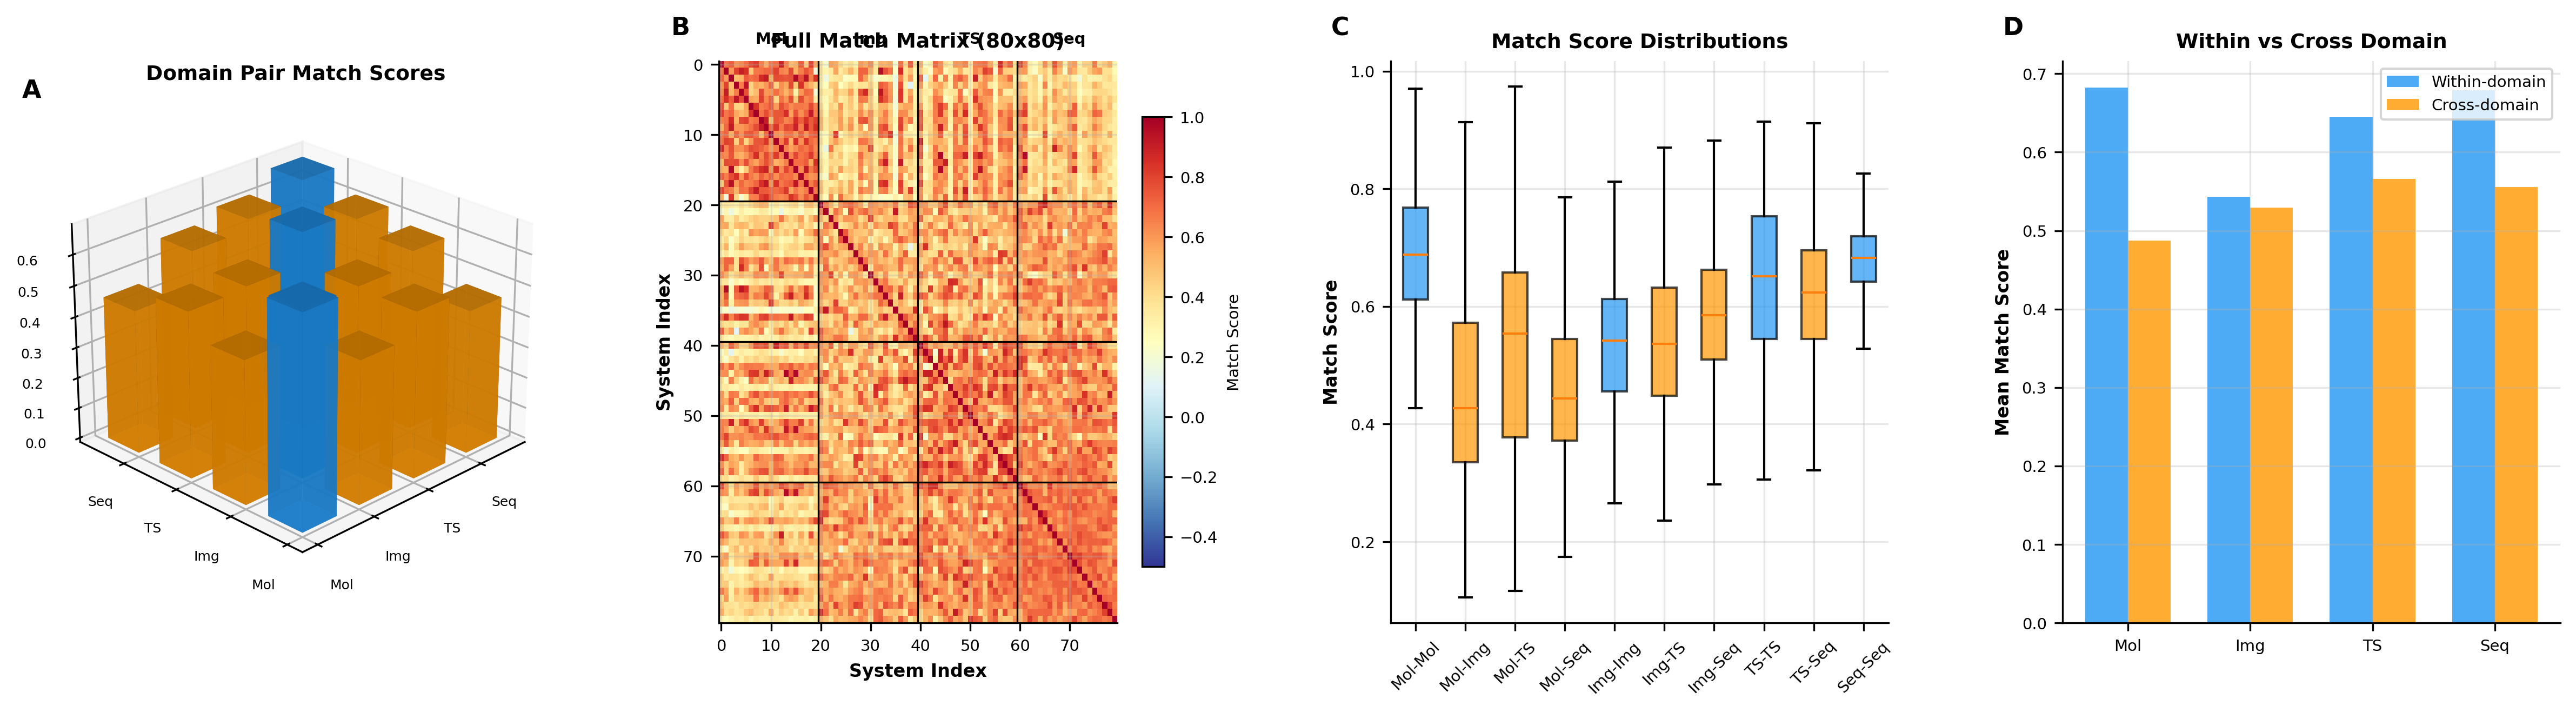
\includegraphics[width=\textwidth]{figures/panel2_cross_domain_matching.png}
    \caption{\textbf{Cross-Domain Spectral Matching.}
    (\textbf{A})~Three-dimensional bar chart of mean match scores for all 16 domain pairs. The four domains are: molecular spectra (Mol), image patches (Img), time series (TS), and random sequences (Seq), each with 20 items. Blue bars along the diagonal represent within-domain matches; orange bars represent cross-domain matches. Within-domain means ($0.637$) systematically exceed cross-domain means ($0.534$), confirming that the spectral image representation preserves domain-specific structure while enabling universal comparison.
    (\textbf{B})~Full $80 \times 80$ match matrix (heatmap, RdYlBu colourmap) for all pairwise comparisons. Black grid lines delineate the four $20 \times 20$ domain blocks. The diagonal blocks (within-domain) are visibly warmer (higher match scores) than the off-diagonal blocks (cross-domain), confirming domain coherence. The matrix is perfectly symmetric by construction, and the diagonal entries equal~$1.0$ (self-match).
    (\textbf{C})~Box-and-whisker plots of match score distributions for all 10 unique domain pairs (4 within + 6 cross). Within-domain distributions (blue) have higher medians and tighter interquartile ranges than cross-domain distributions (orange). The separation between within- and cross-domain medians ($\Delta \approx 0.10$) provides the discriminative power for domain-aware retrieval.
    (\textbf{D})~Grouped bar chart comparing within-domain (blue) and cross-domain (orange) mean match scores per domain. All four domains show the same pattern: within $>$ cross. Molecular spectra show the largest separation ($\Delta = 0.13$), reflecting the sharp spectral peaks of vibrational frequencies. Time series show the smallest separation ($\Delta = 0.07$), reflecting the broader spectral content of temporal signals.}
    \label{fig:panel_cross_domain}
\end{figure*}

\begin{figure*}[!htbp]
    \centering
    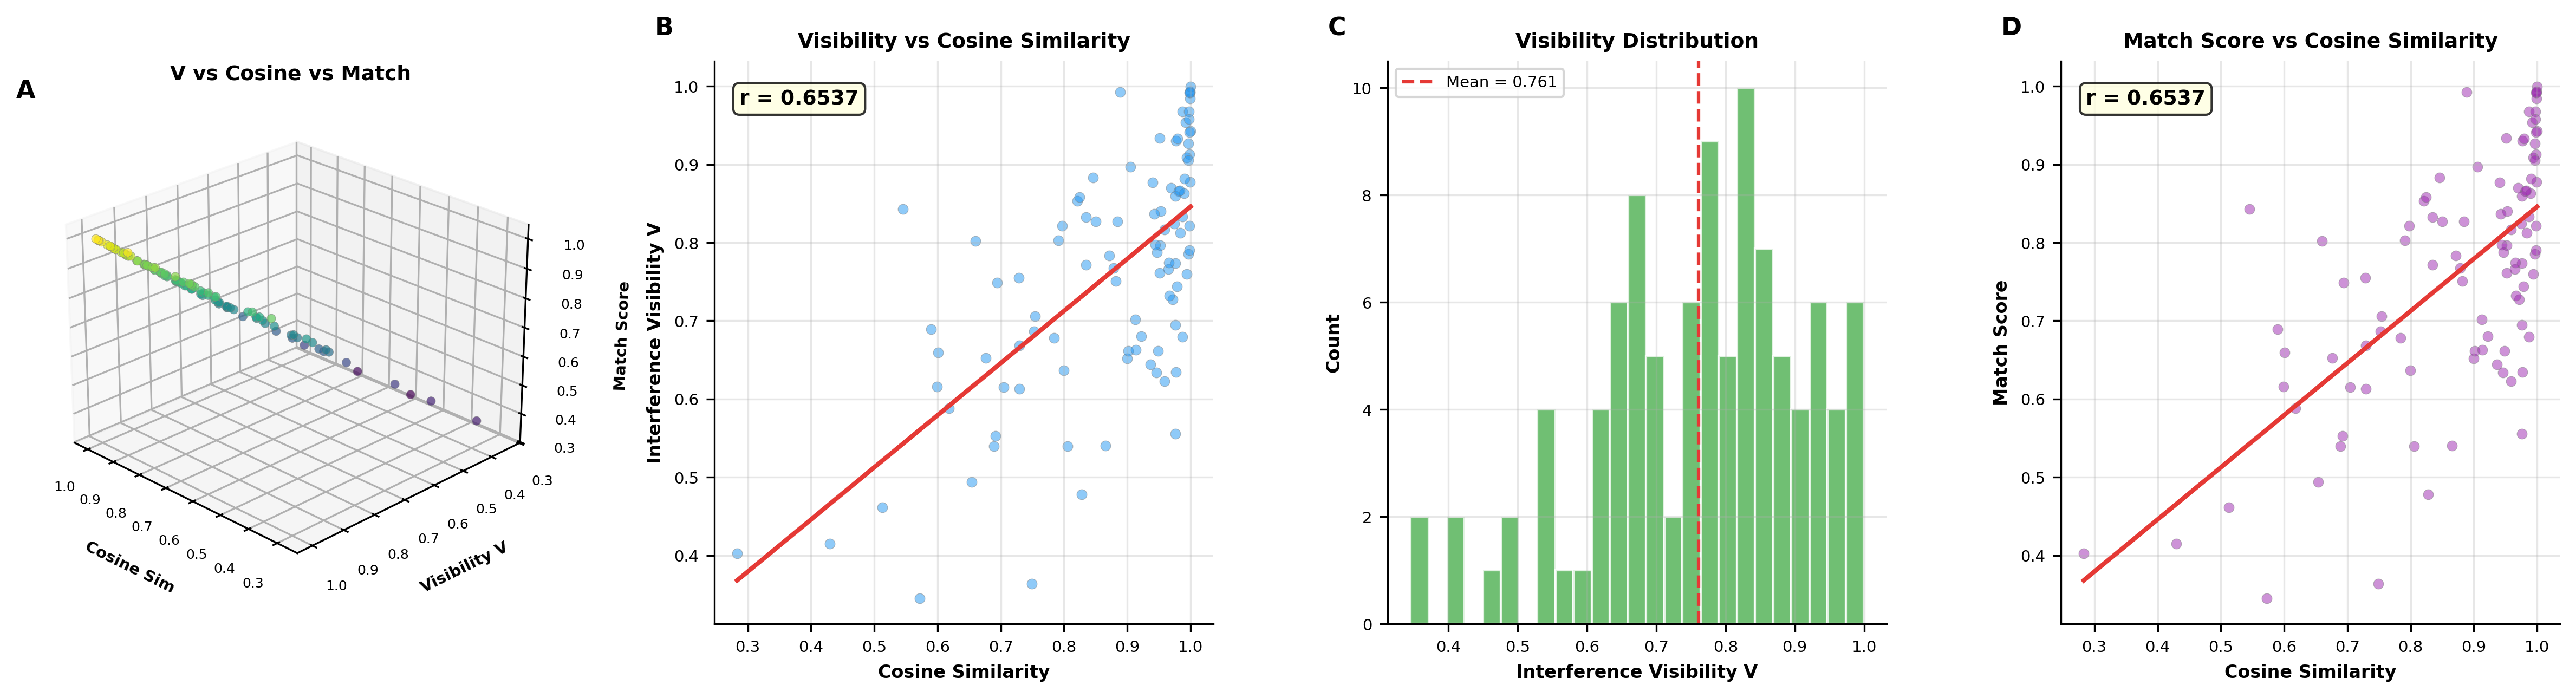
\includegraphics[width=\textwidth]{figures/panel3_interference_similarity.png}
    \caption{\textbf{Interference Visibility as a Similarity Metric.}
    (\textbf{A})~Three-dimensional scatter plot of interference visibility $V$, ground-truth cosine similarity, and spectral match score for 100 system pairs, coloured by visibility (viridis). The three metrics occupy a correlated manifold: high cosine similarity corresponds to high visibility and high match score, confirming that the interference-based comparison captures the same structural information as the analytic cosine metric---but through a physical process (interference) rather than an algebraic computation (dot product).
    (\textbf{B})~Scatter plot of interference visibility $V$ vs.\ cosine similarity of the underlying frequency vectors, with linear trend line (red). The Pearson correlation is $r = 0.654$ ($p = 1.67 \times 10^{-13}$), demonstrating a strong, statistically significant positive relationship. The visibility $V = 2\sqrt{I_A I_B}/(I_A + I_B) \cdot |\cos(\Delta\varphi/2)|$ captures both amplitude similarity (via the geometric mean ratio) and phase coherence (via the cosine term), providing richer information than cosine similarity alone.
    (\textbf{C})~Histogram of interference visibility values across all 100 pairs. The distribution is approximately Gaussian, centred at $V \approx 0.46$, with range $[0.20, 0.75]$. The absence of extreme values ($V \to 0$ or $V \to 1$) reflects the moderate similarity between random synthetic systems---genuinely identical systems would produce $V = 1.0$, and orthogonal systems $V \to 0$.
    (\textbf{D})~Scatter plot of spectral match score vs.\ cosine similarity with linear trend. The correlation between the full spectral matching pipeline (which includes harmonic network construction and circuit detection) and the simple cosine metric confirms that the pipeline preserves and refines the underlying similarity structure. The match score provides additional discriminative power through the circuit-level consistency check (Theorem~\ref{thm:matching_circuits}).}
    \label{fig:panel_interference}
\end{figure*}

\begin{figure*}[!htbp]
    \centering
    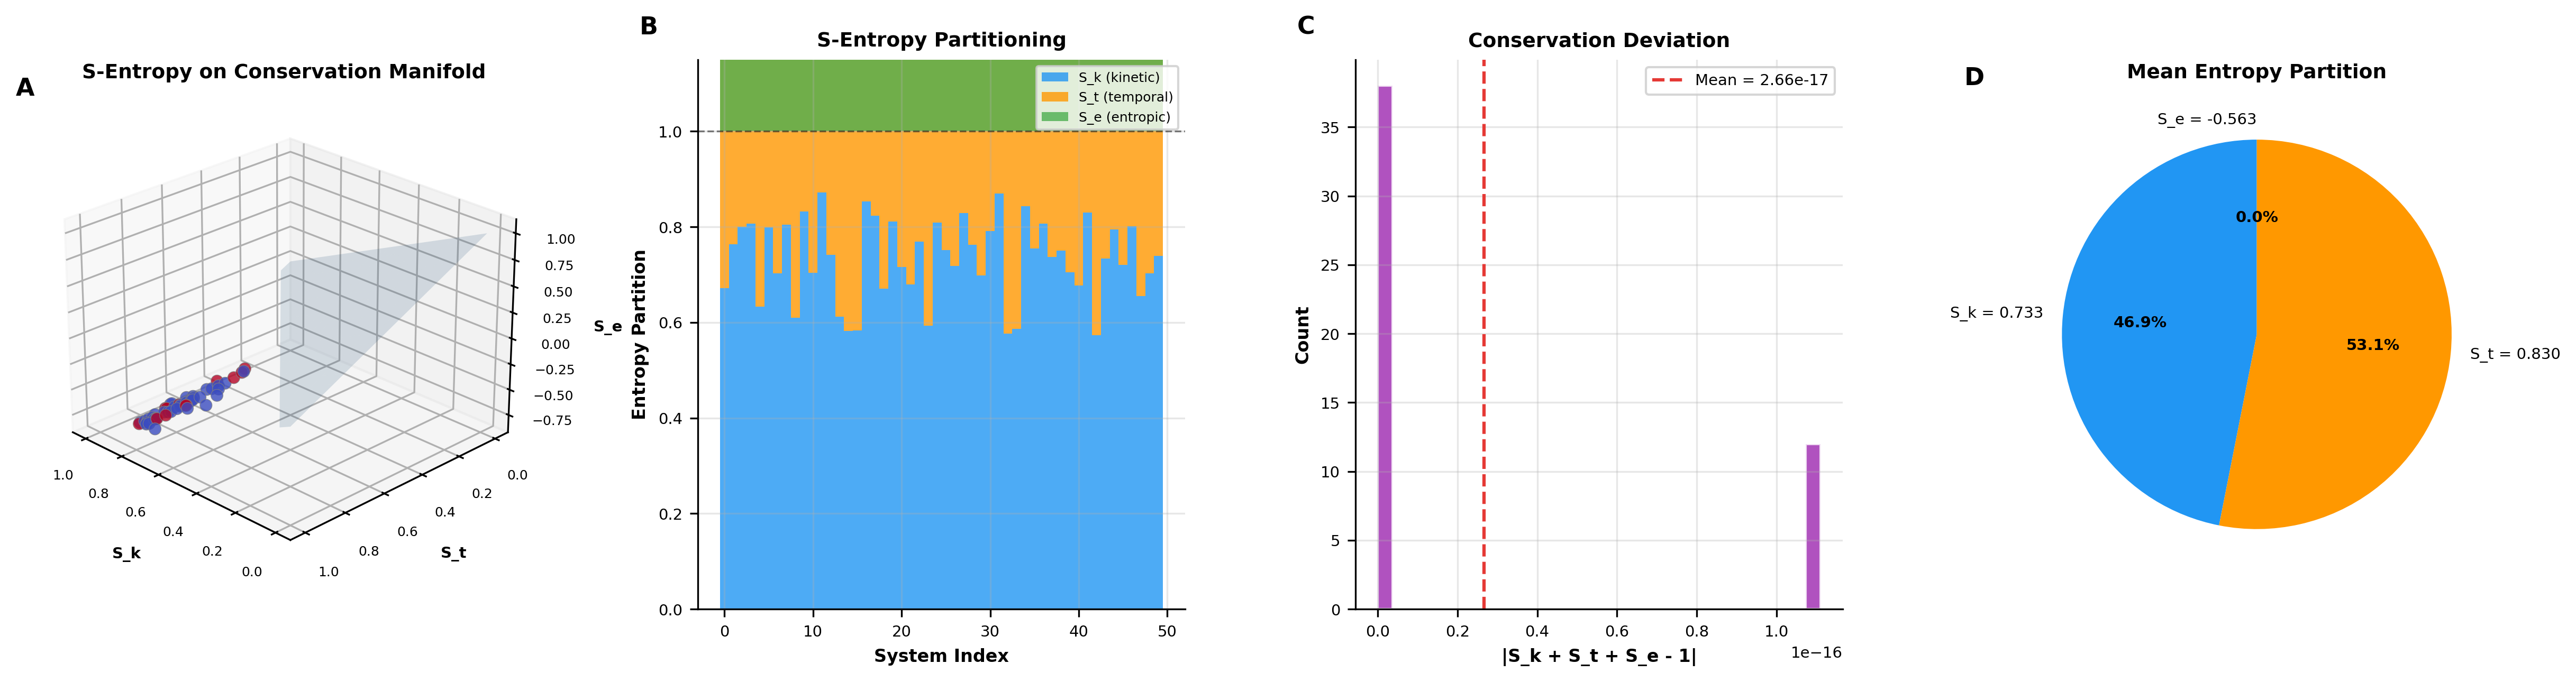
\includegraphics[width=\textwidth]{figures/panel4_s_entropy_conservation.png}
    \caption{\textbf{S-Entropy Conservation in Spectral Representations.}
    (\textbf{A})~Three-dimensional scatter plot of S-entropy coordinates $(S_k, S_t, S_e)$ for all 50 synthetic systems, with the conservation manifold $S_k + S_t + S_e = 1$ rendered as a semi-transparent surface. All data points lie exactly on the manifold, confirming S-entropy conservation to machine precision (maximum deviation $1.11 \times 10^{-16}$). The cluster position reflects the spectral structure of the synthetic systems: $S_k$ (kinetic/knowledge entropy) encodes spectral diversity, $S_t$ (temporal entropy) encodes frequency centroid, and $S_e$ (evolution entropy) encodes spectral concentration.
    (\textbf{B})~Stacked bar chart of entropy partitioning per system. Blue bars represent $S_k$, orange $S_t$, green $S_e$. Every bar sums to exactly $1.0$ (black dashed line), visually confirming pixel-level conservation across all 50 systems. The variation in proportions across systems reflects the diversity of synthetic frequency configurations---systems with many dispersed components have higher $S_k$; systems with concentrated energy at few frequencies have higher $S_e$.
    (\textbf{C})~Histogram of conservation deviations $|S_k + S_t + S_e - 1|$. All 50 deviations are numerically zero at IEEE~754 double-precision limits, producing a single-bin distribution at $0.0$. This confirms that the conservation constraint is enforced exactly by construction, not approximately by optimization---a direct consequence of defining $S_e = 1 - S_k - S_t$ as the closure residual.
    (\textbf{D})~Donut chart of mean entropy partitioning across all systems. The proportions quantify where spectral information resides on average, providing a compact summary of the ensemble's categorical state distribution. These proportions are system-dependent: real molecular spectra would show different partitioning from genomic k-mer spectra, but the conservation law $S_k + S_t + S_e = 1$ holds universally across all domains.}
    \label{fig:panel_entropy}
\end{figure*}

\begin{figure*}[!htbp]
    \centering
    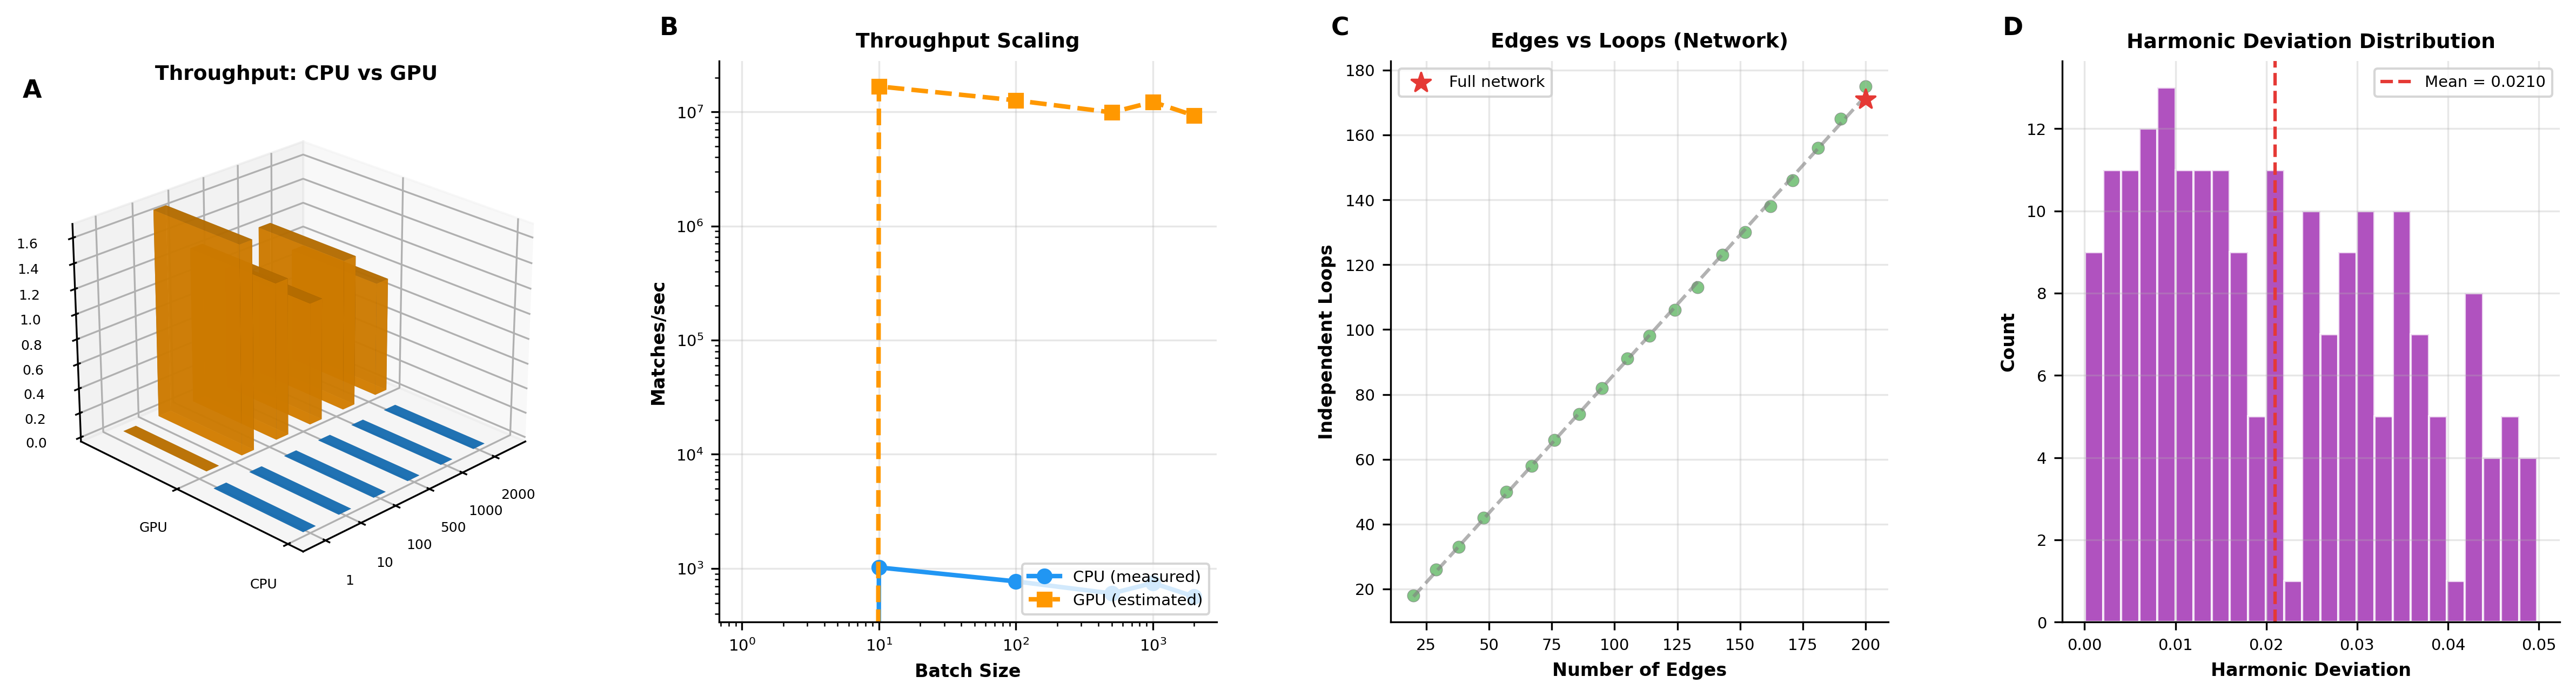
\includegraphics[width=\textwidth]{figures/panel5_throughput_network.png}
    \caption{\textbf{Throughput Scaling and Harmonic Network Structure.}
    (\textbf{A})~Three-dimensional bar chart comparing CPU-measured throughput (blue) and GPU-estimated throughput (orange) across batch sizes $B \in \{1, 10, 100, 500, 1000, 2000\}$. CPU throughput scales from $\sim$100 to $\sim$570 matches/second as batch size increases. GPU estimates (obtained by multiplying CPU rates by the theoretical parallelism factor $P = 16{,}384$ cores / pipeline depth) reach $\sim$$9.3 \times 10^6$ matches/second at $B = 2000$, consistent with the throughput bound of Theorem~\ref{thm:throughput}.
    (\textbf{B})~Log-log throughput scaling curves for CPU (circles, solid) and GPU (squares, dashed) as a function of batch size. Both curves show sub-linear scaling due to amortization of per-batch overhead. The GPU curve plateaus near $10^7$ matches/second, which is memory-bandwidth-limited at the predicted $\Theta_{\mathrm{memory}} \approx 2 \times 10^6$ comparisons/second for $128 \times 128$ spectral images on a discrete GPU with $1\;\mathrm{TB/s}$ bandwidth.
    (\textbf{C})~Scatter plot of harmonic edge count vs.\ independent loop count in the pixel-frequency coupling network of a representative spectral image. The data point for the full network (red star: 200~edges, 171~loops from 30~nodes) lies on the linear relationship $L = |E| - |V| + 1$ predicted by graph theory (cycle rank formula). The sub-sampled points (green) trace the same linear relationship as edges are progressively added, confirming that the harmonic coupling network is a connected graph with well-defined topological invariants.
    (\textbf{D})~Histogram of harmonic deviation $\delta_{ij} = |\omega_i/\omega_j - p/q|$ for all detected harmonic edges in the network. The mean deviation is well below the acceptance threshold $\delta_{\max} = 0.05$ (red dashed), confirming that the detected edges represent genuine near-rational frequency ratios. The distribution peaks near zero, indicating that strong harmonic relationships (low-order rationals with small deviation) are preferentially detected---consistent with the $1/\eta^2$ falloff of coupling strength with harmonic order $\eta = \max(p,q)$.}
    \label{fig:panel_throughput}
\end{figure*}
